% !TeX root = ../main.tex
% Add the above to each chapter to make compiling the PDF easier in some editors.

\chapter{Introduction}
\label{chap:introduction}

\section{Motivation}
\label{sec:introduction_motivation}
Obesity is a huge, growing but preventable problem among children, adolescents and adults in developed countries. Obesity can cause many major diseases like cardiovascular diseases, diabetes or even cancer \cite{Ogden2010, WHO}.

One method to prevent or at least reduce obesity is food logging because it can help to balance the energy intake. Many publications have shown that the action of food logging can be correlated to weight loss \cite{Hollis2008, Burke2011, Svetkey2008}. However, the accuracy of food intake in food diaries is prone to underreporting over all age groups \cite{Livingstone2007}. Especially underreporting is a problem if the goal is to loose weight by balancing the energy intake and activity level. Some approaches relied on expert nutritionists to analyze food images manually or used crowd sourcing to extract nutritional information. Both methods are either costly, inaccurate or slow \cite{Meyers2015}.

It has been proven that taking pictures of food raises a better awareness of the nutritional values of a meal compared to written entries \cite{Zepeda2008} and is also a highly motivating factor for logging food \cite{Kim2010}. Despite the raising trend of sharing pictures of food on social media it is still tedious to actually take pictures of every meal and annotate these images with information about the consumed food items manually.

A possible solution is to extract the nutritional information automatically by using computer vision algorithms and machine learning concepts. In the last few years image recognition and classification made a huge leap forward due to advances in deep learning and increasing computational resources \cite{Szegedy2014}. Computer vision algorithms have come very close to human classification performance and can in some places even surpass the human brain.

Food logging is a perfect example of useful computer vision application because it can potentially increase the accuracy of meal logging and provide a much faster and less cumbersome way of logging food. It allows users to add multiple meal images together so that the diary does not need be opened at every meal. In addition, image recognition enables applications to provide information beyond the knowledge of the user and makes it possible to track the intake of fat or sugar and even warn the user of possible harmful allergens.

This thesis provides the foundation for future food logging applications by facilitating the training, segmentation and classification of food images using modern computer vision algorithms and machine learning models.

\section{Challenges of Food Recognition}
\label{sec:introduction_challenges}

Image recognition has advanced tremendously over the last years. The latest winner of the ImageNet challenge 2015 \cite{Russakovsky2015} achieved a top-5 localization error of only 8.9\% on 1000 different classes with a 150 layer deep neural network \cite{He2015}. Nevertheless, there is still not a single comprehensive, publicly available food classification tool. The best approach so far only achieved a mere 79\% accuracy on a 101 class food dataset \cite{Meyers2015}.

The following section will provide reasons why food recognition is indeed much more challenging than normal object recognition.

The information a useful computer vision aided food intake diary has to extract can be structured into two categories which both pose a challenge for any potential application:

\subsection*{Classification}

\subsubsection{Quantity of Food Types}
The goal of the classification task is to predict the food category as accurately as possible with a preferably complete set of image categories which poses the first problem. Building a classifier for all plane types is relatively easy as the number of possible plane types is limited. The number of different food items, however, is nearly unlimited. There are so many variations of food that it is not possible to train a classifier on all items but for accurate nutrition information extraction it is extremely important to be able to differentiate between different sorts of food items. The nutritional values of a slice of brown bread are different than those of a slice of white bread.

\subsubsection*{Food Parameters}
Another problem for food image classification is that food can be parametrized with different toppings, different kind of sauces or varying methods of preparation. It is very hard to take these food parameters into account because of the huge variety of different parameters. Not only can they completely change the appearance of the food item they also have a huge impact on the nutritions. Salads can be very healthy but combining a salad with an unhealthy topping entirely changes the healthiness of the dish.

\subsubsection*{Intraclass Variance}
The major problem for food classification, however, is the huge intra class variance. Even the same kind of food can look completely different depending on preparation, ingredients and presentation. Normal objects in image recognition tasks mostly appear in some kind of standardized form. Cars for example always include some common features that are easy to distinguish. Figure \ref{fig:intraClassVariance} shows that even a food type that is normally very similar in appearance can have many visually different appearances. 

\begin{figure}[htb]
\centering
\hspace{\fill}%
\subfloat{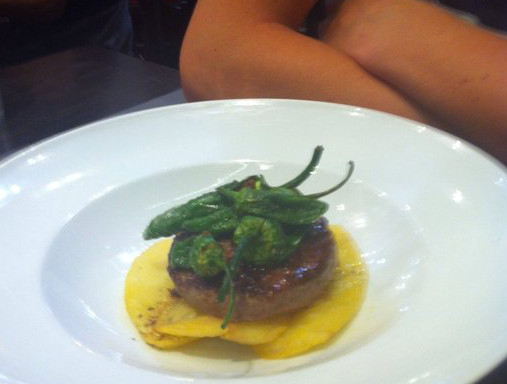
\includegraphics[width=30mm]{data/images/introduction/sameClass1}}
\hspace{\fill}%
\subfloat{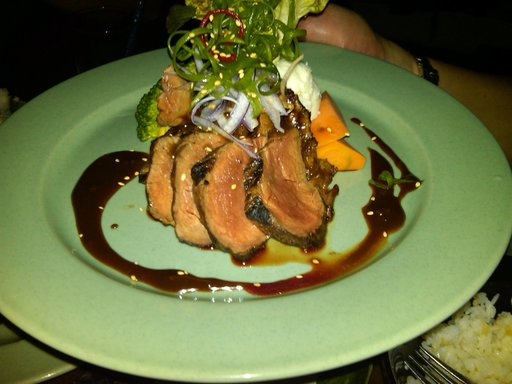
\includegraphics[width=30mm]{data/images/introduction/sameClass2}}
\hspace{\fill}%
\subfloat{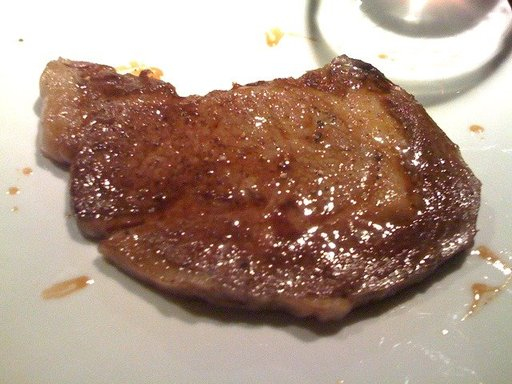
\includegraphics[width=30mm]{data/images/introduction/sameClass3}}
\hspace{\fill}%
\subfloat{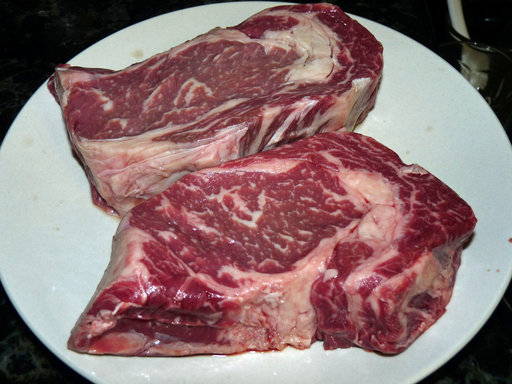
\includegraphics[width=30mm]{data/images/introduction/sameClass4}}

\caption{Examples for intra class variance. Every image shows a "steak" but the visual appearance varies greatly.}
\label{fig:intraClassVariance}
\end{figure}

\subsubsection*{Interclass Variance}
There is a tradeoff between the granularity of a food classifier and its accuracy for the nutrition problem. On one side, there are problems with items that look very different, but are not. On the other side, there are food items which tend to look almost the same, but are different. It is difficult to find a classifier that is able to recognize different preparations of a steak as a "steak" on the one side but is also able to determine the difference between a hamburger and a cheeseburger because the latter has more calories.

\subsubsection*{Unobservable Details}
Even if a future system might solve all aforementioned problems there is still a problem even the most sophisticated image recognition systems can not solve alone. It is not possible to analyze parts of the food that can not be seen. Even expert nutritionists are not able to determine from an image alone what sort of fat or sugar was used for cooking and if this food item contains some kind of stuffing that changes the whole nutritional value. Systems might leverage context information in the future to approximate the "hidden values" by taking additional information like position, time or past preference into account. It is also possible that in coming years smart devices will have build in spectrometers that can be used to analyze the chemical composition of the food \cite{Krem}.

\subsection*{Quantity Estimation}
Unfortunately, a successful classification is not sufficient enough to deduct accurate nutritional information. It is also important to extract some kind of quantity information. For this, the image has to be segmented into different food parts because each food item has different nutritional values. Image segmentation alone is a difficult problem. Food image segmentation can be even harder because food items often lack clearly distinctive parts. A normal landscape image is easily separated into different parts but food items are often similar in color and share a common edge because the contrast between parts is usually very low. 

In addition, food items are often obstructed from each other and may sometimes not even be visible at all like contents of a soup or food scalloped with cheese. But even with a perfectly separated image it is still difficult to get actual quantitative measurements about the items. Meal size area estimation is possible and was implemented for this thesis but for most foods {(other than pizza)} the area alone is not sufficient inasmuch as food usually has some kind of 3-dimensional shape. However, the approximation of volume and depth from single images is very challenging and not nearly as advanced as image recognition is. Models that are used to estimate depth and volume are trained on images of indoor areas \cite{Eigen2015} and not on small objects where absolute error is much more significant than on large objects. Meyers et al. incorporated such volume estimation and achieved a mean error that is still to high for real world scenarios \cite{Meyers2015}. 

\section{Outline}
This thesis is structured into 7 chapters. Chapter \ref{ch:relWork} outlines previous works on food recognition including information about food datasets, existing systems and common algorithms which are then further explained in chapter \ref{ch:theory}. This chapter includes common concepts of machine learning and computer vision. Chapter \ref{ch:experimental_setup} provides information about data preprocessing steps, algorithmic variations and the experimental setup. Chapter \ref{ch:implementation} describes the implementation and architecture of the proposed application. Results are then accumulated and discussed in chapter \ref{ch:discussion}. Lastly, the results are summarized in chapter \ref{ch:conclusion} and advice for future work is given.
